\documentclass[.../bericht]{subfilies}

\begin{document}
  \chapter{Grundlagen}
    \section{Streuung}

      Für die Untersuchung von Atomen und Molekülen werden oft Streuprozesse verwendet. Drei der wichtigsten sind die Compton-Streuung, die Rayleigh-Streuung und die in diesem Versuch verwendete Raman-Streuung.


      \subsection{Compton-Streuung}
      \label{ssec:Compton-Streuung}


      	Der 1922 von Arthur Holly Compton entdeckte Compton-Effekt nutz die Teilcheneigenschaften von Photonen aus und ist damit auch immer wieder ein Musterbeispiel für den Welle-Teilchen Dualismus des Lichtes. Bei diesem Streuprozess trifft Röntgenstrahlung der Wellenlänge $\lambda_0$ auf ein Material. Dabei wird ein Teil der Photonen mit einer größeren Wellenlänge $\lambda_S> \lambda_0$ gestreut. Die Wellenlängenverteilung hängt dabei primär vom Streuwinkel und nur sekundär vom Streumaterial ab. \\
        Um diesen Effekt zu erklären betrachtet man ein Photon der Energie $E=h\nu$ und dem Impuls $p=\hbar k$, das elastisch mit einem schwach gebundenen Elektron zusammenstößt. Wir nehmen an, dass die Bindungsenergie des Elektrons $E_B<<h\nu$ und dass das Elektron sich vor dem Stoß in Ruhe befand. Damit gilt für die Impulserhaltung:
        \begin{equation}
          h\nu_0+e^- \rightarrow h\nu_S+e^-(E_{kin})
          \label{eq:impulserhaltung}
        \end{equation}
        Da die Photonen sich natürlich mit Lichtgeschwindigkeit bewegen und auch das gestoßene Elektron eine hohe Geschwindigkeit besitzt muss relativistisch gerechnet werden. Des Weiteren werde angenommen, dass die Photonen aus der x-Richtung einfallen und in die x-y-Ebene gestreut werden. Daraus folgt für den Energiesatz mit $\beta=v/c$:
        \begin{equation}
          h\nu_0=h\nu_S+E^e_{kin}
          \label{eq:energiesatz}
        \end{equation}
        \begin{equation}
          E^e_{kin}=\frac{m_0c^2}{\sqrt{1-\beta^2}}-m_0c^2=(m-m_0)c^2
          \label{eq:energie}
        \end{equation}
        Durch die Impulsbetrachtung erhält man:
        \begin{equation}
          \hbar k_0=\hbar k_S +p_e \\
          \label{eq:impulssatz}
        \end{equation}
        mit
        \begin{equation}
          p_e=\frac{m_0 v}{\sqrt{1-\beta^2}}
          \label{eq:impuls}
        \end{equation}
        Mit $\phi$ als Winkel zwischen Einfalls- und Streurichtung erhält man nach einigen Umformungsschritten aus \cref{eq:energiesatz} und \cref{eq:impulssatz} die Compton-Streuformel:
        \begin{equation}
          \lambda_S-\lambda_0=2\lambda_csin^2(\frac{\phi}{2}
          \label{eq:streuformel}
        \end{equation}
        mit
        \begin{equation}
          \lambda_c=\frac{h}{m_0c}=2.4262\cdot10^{-12}m
          \label{cwellenl}
        \end{equation}
        als Compton-Wellenlänge des Elektrons. Diese zeigt die Wellenlängenänderung $\Delta \lambda =\lambda_S -\lambda_0$ bei dem Streuwinkel $\phi=\pi/2$. \\
        Dividiert man die Compton-Wellenlänge durch $\lambda_0$, so sieht man dass das Verhältnis der $h\nu_0$ zur Ruheenergie des Elektrons $m_0c^2$ dem Verhältnis $\lambda_c/\lambda_0$ entspricht.
      \begin{equation*}
      \frac{\lambda_c}{\lambda_0}=\frac{h}{m_0c\lambda_0}=\frac{h\nu_0}{m_0c^2}
    \end{equation*}
      Damit lässt sich durch Messung von $\lambda_S$ und $\phi$, bei bekanntem $m_0$, $\lambda_c$ und h bestimmen. Falls an etwas anderem als Elektronen gestreut wird, wie zum Beispiel Protonen oder Neutronen, kann, mit dem Literaturwert von h auch die Ruhemasse des Streuers bestimmt werden.\\
      \cite{dem:exp3}

    \subsection{Rayleigh-Streuung}
  	\label{sec:Rayleigh-Streuung}

      Die zweite wichtige Streuung ist die Rayleigh-Streuung. Diese ist eine elastische Streuung von Licht an Teilchen, die viel kleiner sind als die Wellenlänge des Lichtes und aufgrund ihrer Entfernung nicht miteinander wechselwirken. Sie tritt daher vor allem in Gasen, wie zum Beispiel Luft auf. Die Rayleigh-Streuung ist dafür verantwortlich, dass der Himmel tagsüber blau und am Abend orange ist. Rayleigh-Streuung kann auch auftreten wenn die Streuer in einer Flüssigkeit gelöst sind oder sich als Fremdatome in Festkörpern befinden. \\
      Die einfallenden Photonen regen die Elektronen in den Streuern an. Dadurch entsteht ein Dipolmoment, das als Hertzscher Dipol wieder Wellen der gleichen Wellenlänge aussendet. Für das Dipolmoment gilt:
      \begin{equation}
        p=\alpha E
        \label{eq:dipol}
      \end{equation}
      mit der Polarisierbarkeit $\alpha$. Damit Rayleigh-Streuung auftreten kann müssen die Streuer unregelmäßig verteilt sein, da eine fest Phasenbeziehung zwischen den Streuwellen und der einfallenden Strahlung besteht. Aus der zufälligen Verteilung der Streuer folgt die Inkohärenz des gestreuten Lichts. \\
      Für den differentiellen Wirkungsquerschnitt der Rayleigh-Streuung, mit V als Gasvolumen, N als Teilchendichte, n($\lambda$) als Wellenlängen abhängiger Brechungsindex und $\theta$ als Streuwinkel, ergibt sich:
      \begin{equation}
        \sigma(\theta)=\frac{2\pi^2 V}{N\lambda^4}(n^2(\lambda)-1)^2(1+cos^2\theta)
        \label{eq:streuquerschnitt}
      \end{equation}
      Hierbei ist die rechte Seite der Gleichung die Rayleighsche Streufunktion. \\

      Die Streustrahlung besteht aus einem senkrecht ($i_1$) und einem parallel ($i_2$) polarisierten Anteil. $i_1$ ist proportional zur eins in der zweiten Klammer und $i_2$ ist proportional zu $cos^2\theta$. Damit ist $i_2=0$ für $\theta=\pi/2$, $3\pi/2$, daraus folgt, dass das Streulicht vollständig polarisiert ist. Demnach ist das Streulicht für $i_1=i_2$, bei $\theta=0$, $\pi$, unpolarisiert.

      \begin{figure}[H]
        \begin{center}
          \fbox
          {
          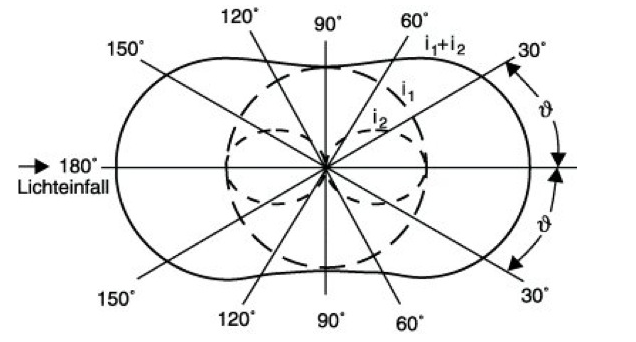
\includegraphics[scale=1]{figures/rstreuung}
          }
          \caption{Intensitätsdiagramm der beiden Polarisationsrichtungen $i_1$ und $i_2$ der Rayleigh-Streuung in Abhängigkeit des Streuwinkels $\theta$. \cite{spektrum:rayleigh}
          }
        \end{center}
      \end{figure}
      Wenn ein unpolarisierter Strahl der Intensität $I_0$ und der Wellenlänge $\lambda$ auf ein Molekül trifft so gilt für die Intensität der gestreuten Strahlung:
      \begin{equation}
        I=I_0\frac{8\pi^4 \alpha^2}{\lambda^4 R^2}(1+cos^2\theta)
        \label{eq:rayleighi}
      \end{equation}
      mit der Polarisierbarkeit $\alpha$, dem Streuwinkel $\theta$ und dem Abstand vom Streuer R.\\
      Den totalen Streuquerschnitt erhält man indem man $\sigma(\theta)$ über alle Streurichtungen integriert. Wird dieser durch V dividiert folgt der Rayleighsche Streukoeffizient.
      \begin{equation*}
        b=\frac{8\pi^3}{3N\lambda^4}[n^2(\lambda)-1]^2
      \end{equation*}
      Da die Streuintensität stark von $\lambda^{-4}$ abhängt wird blaues Licht ca. 10 mal stärker gebrochen als rotes Licht, was wie am Anfang erwähnt zur Färbung des Himmels führt.
      \cite{cosmos} \cite{wiki:rayleigh} \cite{spektrum:rayleigh}

    \subsection{Raman-Streuung}
    \label{ssec:Raman-Streuung}

      Bei der Raman-Streuung findet nun ein inelastischer Streuprozess an Molekülen statt. Die Raman Streuung ist deutlich schwächer als die Rayleigh-Streuung erlaubt aber auch mehr Rückschlüsse auf die Struktur der Moleküle. Beim Raman-Effekt hebt ein Photon der Energie $\hbar \omega_0$ vom Anfangzustand $E_k$ in den höheren Zustand $E_i$. Das dabei gestreute Photon hat nun die Energie $\hbar \omega_s$. Damit gilt:
      \begin{equation*}
        \Delta E= \hbar (\omega_0-\omega_s)=E_i-E_k
      \end{equation*}
      Wird nun monochromatisches Licht auf die Molekülprobe gelenkt, sieht man in Spektrum noch andere Strahlungen, zusätzlich zur elastisch gestreuten Wellenlänge $\lambda_0$, der Rayleigh-Streuung. Die Stokes-Strahlung entsteht auf der langwelligen Seite von $\lambda_0$  durch Rotations-Schwingungs-Energiedifferenzen der Moleküle. Desweiteren entsteht auf der kurzwelligen Seite von $\lambda_0$ wenn die streuenden Moleküle bereits angeregt sind und in den Grundzustand zurückfallen, siehe und \cref{fig:oszillator}.
      \begin{figure}[tb]
        \begin{center}
          \fbox
          {
            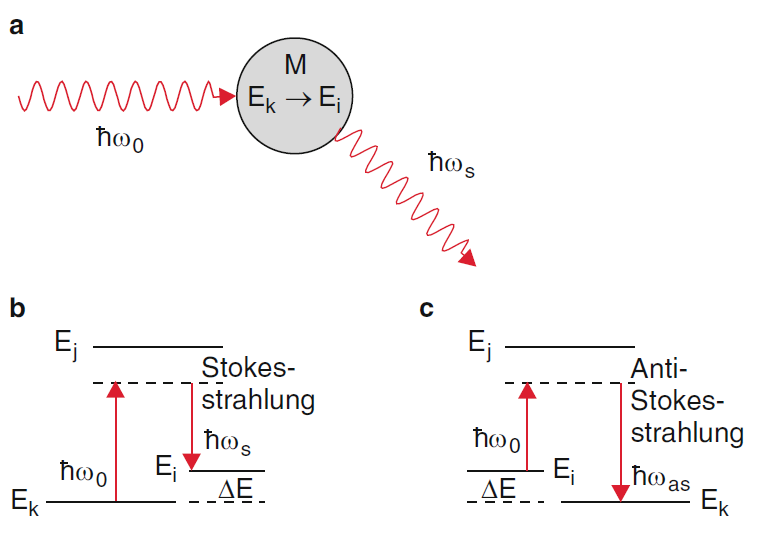
\includegraphics[scale=0.5]{figures/rayleighphoton}
            }
            \caption{a) Streuprozess des Photons an einem Molekül; b) Energieniveaus des Moleküls bei Stokes- und Anti-Stokes-Strahlung. \cite{dem:exp3}
          }
          \label{fig:anti-stokes}
        \end{center}
      \end{figure}

      \begin{figure}[tb]
          \begin{center}
          \fbox
          {
            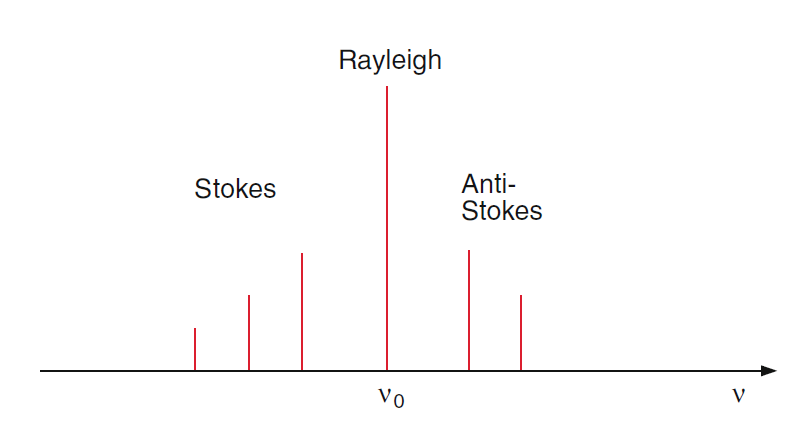
\includegraphics[scale=0.5]{figures/ramanspektrum}
          }
          \caption{Relative Position der Rayleigh-, Stokes- und Anti-Stokes-Intensitätsmaxima zueinander, über Frequenz aufgetragen, mit Stokes im niederfrequenten und Anti-Stokes im höher frequenten Bereich. \cite{dem:exp3}
          }
          \label{fig:schema}
        \end{center}
      \end{figure}

      Bei der klassischen Beschreibung des Raman-Effektes überlagert sich das induzierte Dipolmoment der Rayleigh-Streuung aus \cref{eq:dipol} mit einem bereits vorhandenen Dipolmoment des Moleküls $p_{el}^0$ zu:
      \begin{equation*}
        p_el=p_{el}^0+\widetilde{\alpha} E
      \end{equation*}
      \begin{equation*}
      p_{el}=-e\sum_i r_i+e\sum_k Z_k R_k
      \end{equation*}
      Mit $r_i$ als Elektronen- und $R_k$ als Kern-Koordinaten.
      Die schnelle Elektronenbewegung wird herausgemittelt und die Kern-Auslenkung $Q_k=|R_k-R_k^0|$ für kleine Amplituden als harmonische Schwingung betrachtet $Q_n(t)=Q_{n0}\cdot cos\omega_n t$. Mit einer Taylorentwicklung und einigen Umformungen folgt:
      \begin{equation}
        p_{el}=p_{el}^0+\sum_n (\frac{\partial p_{el}}{\partial Q_n})_0 Q_{n0}cos\omega_n t+\widetilde{\alpha}(0) E_0 cos\omega t+(\sum_n (\frac{\partial \alpha_{ij}}{\partial Q_n})_0 Q_{n0}cos(\omega \pm \omega_n)t)\frac{E_0}{2}
        \label{eq:gesamtdipolmoment}
      \end{equation}
      Der erste Term beinhaltet das intrinsische Dipolmoment des Moleküls und der zweite den Anteil, der mit der Molekülschwingung oszilliert. Dieser ist für das Infrarotspektrum verantwortlich. Die letzten beiden Teile geben den Anteil des Dipolmomentes an, der durch die einfallende Welle induziert wird.\\
      Die Stärke des dritten Terms (Rayleigh-Streuung) hängt von der Polarisierbarkeit des Moleküls gegenüber der Richtung des Wellenvektors $E_0$.
      Die Amplitude der Stokes- $(\omega-\omega_n)$ und Anti-Stokes-Streuung $(\omega-\omega_n)$ hängt von der Polarisierbarkeit im Verhältnis zur Kernauslenkung $(\partial \alpha_{ij} / \partial Q_n)$ ab. Man kann aus der Verschiebung der Stokes- und Anti-Stokes-Linien die die Schwingungsfrequenzen des Moleküls bestimmen. Höhere Schwingungsordnung treten bei genügend hoher Auflösung mit abnehmender Intensität auf. Das Verhältnis von Stokes und Anti-Stokes lässt sich mithilfe der Boltzmann-Verteilung in einer quantenmechanischen Betrachtung bestimmen. Diese liefert das Ergebnis:
      \begin{equation}
        \frac{I_{Stokes}}{I_{Anti-Stokes}}=\frac{(\omega-\omega_n)^4}{(\omega+\omega_n)^4}exp(-\hbar \omega_n/ k_B T)
        \label{eq:stokesvergleich}
      \end{equation}
      % hier
      mit der Boltzmann-Konstante $k_B$ und der Temperatur T. Also kann man aus dem Stokes-, Anti-Stokes-Verhältnis die Temperatur der Moleküle bestimmen.
      Des Weiteren verschwindet für homonukleare Moleküle das IR-Spektrum, da $\partial p_{el}/ \partial Q_n)=0$, aber das Raman-Spektrum $(\partial \widetilde{\alpha} / \partial Q) \neq 0$ bleibt erhalten. Aus der Raman-Komponente $(\partial \widetilde{\alpha} / \partial Q)$ kann man die Abhängigkeit der Polarisierbarkeit von den Normalkoordinaten bestimmen. Daraus folgen dann wiederum die Ladungsverschiebungen und Rückstellkonstanten der Molekülschwingungen. \\
      Vergleicht man IR und Raman-Spektroskopie stellt man einige Unterschiede fest. Beim Raman-Effekt wird das Photon nur gestreut während es bei der IR-Spektroskopie vom Molekül absorbiert wird. Die Vibration des Moleküls ist Raman-Aktiv wenn sie eine Veränderung in der Polarisierbarkeit bewirkt, daher wird kein permanentes Dipolmoment benötigt. Dagegen ist eine Vibration IR-Aktiv wenn sie eine Veränderung im Dipolmoment bewirkt. Außerdem kann bei der IR-Spektroskopie die Probe nicht in Wasser gelöst werden, da Wasser nur eine sehr geringe Durchlässigkeit für IR-Licht hat. Für die Schwingungen der Moleküle gilt: symmetrische Valenzschwingung, IR-inaktiv/ Raman-aktiv; antisymmetrische Valenzschwingung, IR-aktiv/ Raman-inaktiv; zwei Deformationsschwingungen, IR-aktiv/ Raman-inaktiv. \\
      Über den Depolarisationsgrad der Raman-Linien können Aussagen über die Symmetrie der Schwingungsmoden getroffen werden. Der Depolarisationsgrad ist definiert durch:
      \begin{equation}
        \rho=\frac{3\gamma'^2}{45{\alpha'^2}+4\gamma'^2}
        \label{eq:depolarisation}
      \end{equation}
      mit $\alpha'$ als isotroper und $\gamma'$ als anisotroper Anteil. $\rho$ liegt also für die Raman-Linien im Wertebereich: $0\leq \rho \leq \frac{3}{4}$. Für $\rho=0$ sind die Moleküle vollständig isotrop ($\gamma'=0$) und die Raman-Linien sind vollständig polarisiert. Für $\rho=\frac{3}{4}$ sind die Moleküle vollständig anisotrop ($\alpha'=0$) und die Raman-Linien sind vollständig depolarisiert. $\rho<\frac{3}{4}$ nur bei der Existenz von totalsymmetrischen Eigenschwingungen wegen $\alpha'^2>0$. Also kann man aus dem Depolarisationsgrad Rückschlüsse auf die Molekülstruktur treffen.\\
      \cite{raman-ir} \cite{molekuel}

      % hier
  \section{Schwingung im Molekül}

    Moleküle besitzen drei Translations-Freiheitsgrade, sowie drei Rotations-Freiheitsgrade. Zusätzlich hat ein Molekül noch Freiheitsgrade durch Schwingungen in den Bindungen zwischen den Atomen. Je nach Bindung und Molekül sind Streckung und Stauchung möglich, sowie Schwingungen orthogonal zur Bindungsrichtung.  Damit können Freiheitsgrade abhängig von der Anzahl der Bindungen und Bindungsart dazukommen. Die einfachste Schwingung ist der harmonische Oszillator zwischen zwei Atomen. Sei n die Schwingungsquantenzahl, k die Federkonstante, $m_{1/2}$ die Massen der Atome und $\omega$ die Kreisfrequenz der Schwingung, dann gilt
    \begin{equation}
      E=(n+\frac{1}{2})\hbar \sqrt{k(\frac{1}{m_1}+\frac{1}{m_2})}=(n+\frac{1}{2})\hbar \omega
      \label{eq:harmonischeroszi}
    \end{equation}
    Die Regel für die Schwingungsübergänge lautet $\Delta n= \pm 1$ und der Abstand zwischen den Energieniveaus ist identisch. Für die Frequenz gilt:
    \begin{equation*}
      \omega_=\sqrt{k/\mu}
    \end{equation*}
    mit der reduzierten Masse $\mu=\frac{m_1m_2}{m_1+m_2}$.\\
    Für reale Moleküle muss der harmonische Oszillator angepasst werden, da die Bindungskräfte eine unbegrenzte Dehnung und die Abstoßungskräfte zwischen den Atomen eine unbegrenzte Stauchung verhindern. E in Abhängigkeit von $\Delta r$, als Auslenkung vom Gleichgewichtspunkt, wird nun mithilfe der Dissoziationsenergie D und einer Molekülspezifischen Konstante a beschrieben.
    \begin{equation}
      E=D_e[e^{-\alpha \Delta r}-1]^2=\hbar \omega(\frac{1}{2}+n)-\alpha \hbar \omega (\frac{1}{2}+n)^2+...
      \label{eq:anharmonischerosz}
    \end{equation}
    % hier
    Den Verlauf des (An)harmonischen Oszillators sieht man in \cref{fig:oszillator}.
    Beim anharmonischen Oszillator sind die Niveaus nicht mehr äquidistant und für die Auswahlregel gilt $\Delta n= \pm 1, \pm 2, \pm 3$.\\
    \cite{schwingungsspek}

    \begin{figure}[tb]
      \centering
      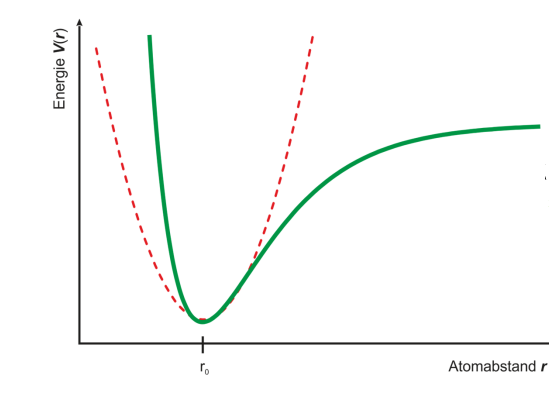
\includegraphics[scale=0.5]{figures/oszillator}
      \caption{DIe Energie aufgetragen über dem Atomabstand. Die gestrichelte Linie zeigt den harmonischen und die grüne den anharmonischen Oszillator. \cite{schwingungsspek}}
      \label{fig:oszillator}
    \end{figure}

  \section{Komponenten des Versuchsaufbaus}

    \textbf{Nd:Yag-Laser:}\\
    Der in diesem Versuch verwendete Laser besteht aus einem Neodynium (Nd) dotierten Yttrium Aluminium Garnet (YAG) Kristall. Der Nd:YAG-Laser ist ein 4-Niveau Doidenlaser, das heißt der Laserkristall wird  gleichzeitig als Resonator verwendet, wie es für Diodenlaser typisch ist. Der Laser emittiert eigentlich Licht der Wellenlänge 1064 nm. Allerdings wird die Wellenlänge mithilfe einer Frequenzverdopplung auf 532 nm verkürzt, um sichtbares grünes Licht zu erhalten.\\
    \cite{ndyag}
    \medskip

    \textbf{Kerbfilter:}\\
    Ein Kerbfilter, kann eine Bestimmte Frequenz aus einem Spektrum filtern. In diesem Versuch wird er verwendet um den Rayleigh-Peak zu schwächen, da dieser, wie bereits in \cref{sec:Rayleigh-Streuung} erwähnt, viel stärker ist als die Raman-Peaks.\\
    \cite{wiki:kerbfilter}
    \medskip

    \textbf{Czerny-Turner Spektrometer:}\\
    Da die Fotodioden des CCD-Sensors die Intensität des gesamten Spektrums messen würden und nicht für eine bestimmte Wellenlänge, muss ein Spektrometer eingesetzt werden. In diesem Versuch wird ein Czerny-Turner Spektrometer verwendet um die verschiedene Wellenlängen durchzufahren.

    \begin{figure}[tb]
      \begin{center}
        \fbox
        {
          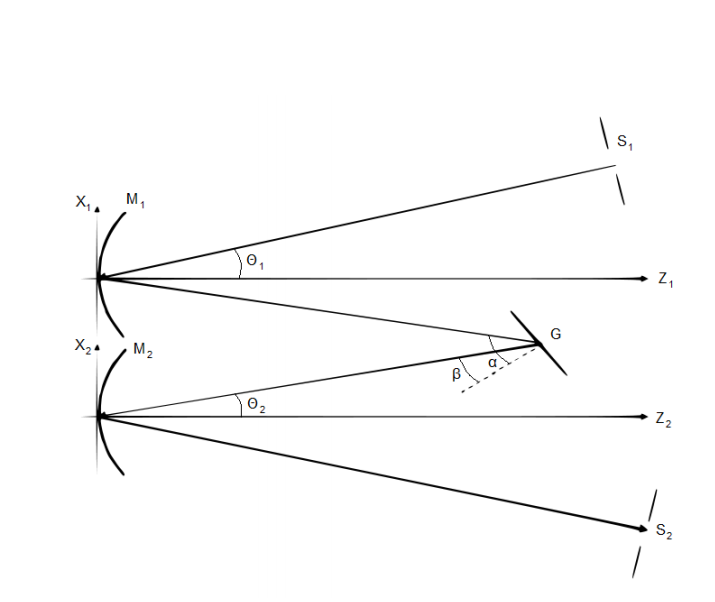
\includegraphics[scale=0.5]{figures/spektrometer}
        }
        \caption{Schematische Darstellung eines Czerny-Turner-Monochromators \cite{czerny}.
        }
        \label{fig:spektrometer}
      \end{center}
    \end{figure}

    Wird das Czerny-Turner-Spektrometer als Monochromator verwendet, wird es wie in \cref{fig:spektrometer} aufgebaut. Der Lichtstrahl tritt durch den Spalt $S_1$ ein, wird vom Kollimator Spiegel $M_1$ kollimiert und auf das Gitter G reflektier. Von dort fällt der Strahl auf den Kameraspiegel $M_2$, dieser fokussiert das Spektrum in der Fokalebene. In dieser Ebene steht auch der Austrittsspalt, durch den das Licht nach draußen fällt. Das Gitter kann durch einen Schrittmotor gedreht werden. Damit kann die Intensität in Abhängigkeit der Gitterstellung aufgetragen werden. Die Skala kann über bekannt Wellenlängen kalibriert werden.
    \cite{czerny}\\
    \medskip

    \textbf{Charge coupled Devices (CCD):}\\
    Der CCD-Sensor wird am Ende des Spektrometers  nach $S_2$ aufgebaut und misst die Lichtintensität. Das Bauteil ist aus mehreren Fotodioden aufgebaut. Je mehr Dioden desto besser die Bildauflösung und je größer die einzelnen Dioden, desto höher die Lichtempfindlichkeit.

    \cite{wiki:ccd}

\end{document}
